\NeedsTeXFormat{LaTeX2e}[1995/12/01]
\documentclass[10pt]{bmcart}
%\documentclass[twocolumn]{bmcart}% uncomment this for twocolumn layout and comment line below
%%% additional documentclass options:
%  [doublespacing]
%  [linenumbers]   - put the line numbers on margins

% Load packages
\usepackage{url}  % Formatting web addresses  
\urlstyle{rm}
\usepackage[utf8]{inputenc} %unicode support
\usepackage{amssymb}
%\usepackage{cite}
\usepackage{graphicx}
\usepackage{multirow}

%% Comment out before submission 
\usepackage[colorinlistoftodos,textsize=small]{todonotes}

%%%%%%%%%%%%%%%%%%%%%%%%%%%%%%%%%%%%%%%%%%%%%%%%%	
%%                                             %%
%%  If you wish to display your graphics for   %%
%%  your own use using includegraphic or       %%
%%  includegraphics, then comment out the      %%
%%  following two lines of code.               %%   
%%  NB: These line *must* be included when     %%
%%  submitting to BMC.                         %% 
%%  All figure files must be submitted as      %%
%%  separate graphics through the BMC          %%
%%  submission process, not included in the    %% 
%%  submitted article.                         %% 
%%                                             %%
%%%%%%%%%%%%%%%%%%%%%%%%%%%%%%%%%%%%%%%%%%%%%%%%%                     

%\def\includegraphic{}
%\def\includegraphics{}

%%% Put your definitions there:
\startlocaldefs
\endlocaldefs


%%%%%%%%%%%%%%%%%%%%%%%%%%%% RESEARCH PAPER %%%%%%%%%%%%%%%%%%%%%%%%%%%%%%%%%%%

%\def \cdkversion {\textbf{2.0}}
\def \cdkversion {v2.0}

\begin{document}

%%% Start of article front matter
\begin{frontmatter}

\begin{fmbox}
\dochead{Research}

% previous titles:
%
% The Chemistry Development Kit (CDK): an open-source Java library for Chemo- and Bioinformatics.
% Recent developments of the chemistry development kit (CDK) - an open-source java library for chemo- and bioinformatics.

\title{The Chemistry Development Kit (CDK): atom typing, rendering, molecular formulas, and substructure searching}

\author[
   addressref={um},                                 % ORCID: 0000-0001-7542-0286
   %corref={aff1},
   %noteref={n1},
   email={egon.willighagen@maastrichtuniversity.nl}
]{\inits{ELW}\fnm{Egon L} \snm{Willighagen}}
\author[
   addressref={nm},
   email={john.may@cantab.net}
]{\inits{JWM}\fnm{John W} \snm{Mayfield}}
\author[
   addressref={uppsala},
   email={jonathan.alvarsson@farmbio.uu.se}
]{\inits{JA}\fnm{Jonathan} \snm{Alvarsson}}
\author[
   addressref={uppsala},
   email={berg.arvid@gmail.com}
]{\inits{AB}\fnm{Arvid} \snm{Berg}}
\author[
   addressref={azg},                                % ORCID: 0000-0001-9491-4134
   email={Lars.A.Carlsson@astrazeneca.com}
]{\inits{LC}\fnm{Lars}~\snm{Carlsson}}
% \author[
%    addressref={jena},
%    email={kai.duehrkop@uni-jena.de}
% ]{\inits{KD}\fnm{Kai} \snm{Dührkop}}
\author[
   addressref={idea},
   email={jeliazkova.nina@gmail.com}
]{\inits{NJ}\fnm{Nina} \snm{Jeliazkova}}
\author[
   addressref={leicester},
   email={shk12@le.ac.uk}
]{\inits{SK}\fnm{Stefan} \snm{Kuhn}}
\author[
   addressref={wi_mit},                             % ORCID: 0000-0002-6940-3006
   email={pluskal@wi.mit.edu}
]{\inits{TP}\fnm{Tomáš}~\snm{Pluskal}}
\author[
   addressref={miquel},                             % ORCID: 0000-0002-4659-1446
   email={mrojas@qca.es}
]{\inits{MRJ}\fnm{Miquel}~\snm{Rojas-Chertó}}
\author[
   addressref={uppsala},
   email={ola.spjuth@farmbio.uu.se}
]{\inits{OS}\fnm{Ola} \snm{Spjuth}}
\author[
   addressref={gilleain},                           % ORCID: 0000-0002-8368-6954
   email={gilleain.torrance@gmail.com}
]{\inits{GT}\fnm{Gilleain} \snm{Torrance}}
\author[
   addressref={um},
   email={chris.evelo@maastrichtuniversity.nl}
]{\inits{CTE}\fnm{Chris T} \snm{Evelo}}
\author[
   addressref={nih},
   email={guhar@mail.nih.gov}
]{\inits{RG}\fnm{Rajarshi} \snm{Guha}}
\author[
   addressref={ebi},
   email={steinbeck@ebi.ac.uk}
]{\inits{CS}\fnm{Christoph}~\snm{Steinbeck}}

\address[id=um]{
  \orgname{Dept of Bioinformatics - BiGCaT, NUTRIM, Maastricht University}, % university, etc
  %\street{Waterloo Road},
  \postcode{NL-6200 MD},
  \city{Maastricht},
  \cny{The Netherlands}
}
\address[id=nm]{
  \orgname{NextMove Software Ltd},
  %\street{D\"{u}sternbrooker Weg 20},
  \postcode{CB4 0EY},
  \city{Cambridge},
  \cny{UK}
}
\address[id=uppsala]{
  \orgname{Department of Pharmaceutical Biosciences, Uppsala University},
  %\street{D\"{u}sternbrooker Weg 20},
  \postcode{751 24},
  \city{Uppsala},
  \cny{Sweden}
}
\address[id=azg]{
  \orgname{AstraZeneca, Innovative Medicines \& Early Development, Quantitative Biology},
  %\street{},
  %\postcode{LE1 7RH},
  \city{Mölndal},
  \cny{SE}
}
% \address[id=jena]{
%   \orgname{Chair for Bioinformatics, Friedrich Schiller University},
%   %\street{},
%   \postcode{07743},
%   \city{Jena},
%   \cny{Germany}
% }
\address[id=idea]{
  \orgname{Ideaconsult Ltd},
  \street{A. Kanchev 4},
  \postcode{1000},
  \city{Sofia},
  \cny{Bulgaria}
}
\address[id=leicester]{
  \orgname{Department of Informatics, University of Leicester},
  %\street{},
  %\postcode{LE1 7RH},
  \city{Leicester},
  \cny{UK}
}
\address[id=wi_mit]{
  \orgname{Whitehead Institute for Biomedical Research}, 
  \street{9 Cambridge Center},
  \postcode{MA 02142},
  \city{Cambridge},
  \cny{USA}
}
\address[id=miquel]{
  \orgname{Química Clínica Aplicada},
  %\street{4 Hanway Place},
  \postcode{43870},
  \city{Amposta},
  \cny{Spain}
}
\address[id=gilleain]{
  %\orgname{Department of Informatics, University of Leicester},
  \street{4 Hanway Place},
  \postcode{W1T 1HD},
  \city{London},
  \cny{UK}
}
\address[id=nih]{
  \orgname{National Center for Advancing Translational Science},
  \street{9800 Medical Center Drive},
  \postcode{MD 20878},
  \city{Rockville},
  \cny{USA}
}
\address[id=ebi]{
  \orgname{Metabolomics and Molecular Informatics, EMBL-EBI},
  %\street{A. Kanchev 4},
  %\postcode{1000},
  \city{Hinxton},
  \cny{UK}
}


%\begin{artnotes}
%\note{Sample of title note}     % note to the article
%\note[id=n1]{Equal contributor} % note, connected to author
%\end{artnotes}

\end{fmbox}% comment this for two column layout

%% The Abstract begins here
\begin{abstractbox}

\begin{abstract}
% Do not use inserted blank lines (ie \\) until main body of text.
\parttitle{Background}
The Chemistry Development Kit (CDK) is a 
widely used open source cheminformatics toolkit, providing data
structures to represent chemical concepts along with methods to
manipulate such structures and perform computations on them. The
library implements a wide variety of cheminformatics algorithms
ranging from chemical structure canonicalization to molecular
descriptor calculations and pharmacophore perception. Over the
last ten years, the code base has grown significantly resulting in
many complex interdependencies among components and poor
performance of many algorithms. 
\parttitle{Results}
We report improvements to the CDK \cdkversion{} since the v1.2 release series,
specifically addressing the increased functional complexity and poor
performance. We first summarize the addition of new, and
improvements to existing functionality that has led to significant
improvement in performance and support for important chemistry
features including atom type perception, substructure searching, molecular
fingerprints, rendering of molecules, and handling of molecular formulas.
Second, we outline how the CDK has evolved with respect to
quality control and the approaches we have adopted to ensure stability, including
a code review mechanism.
\parttitle{Conclusions}
This paper highlights the our continued efforts to provide a community
driven, open source
cheminformatics library, and show that such collaborative projects can exist over
extended periods of time, resulting in a high-quality and performant
library. By taking 
advantage of community support and contributions, we show 
that an open source cheminformatics project can act as a peer reviewed
publishing platform for scientific computing software.
\end{abstract}

\begin{keyword}
\kwd{Java}
\kwd{cheminformatics}
\kwd{bioinformatics}
\kwd{metabolomics}
\kwd{depiction}
\end{keyword}

% MSC classifications codes, if any
%\begin{keyword}[class=AMS]
%\kwd[Primary ]{}
%\kwd{}
%\kwd[; secondary ]{}
%\end{keyword}

\end{abstractbox}
%
%\end{fmbox}% uncomment this for twcolumn layout

\end{frontmatter}


%%%%%%%%%%%%%%%%
%% Background %%
%%
\section*{Background}

The open source cheminformatics community has made significant steps
forward recently~\cite{OBoyle2011b} as evidenced by the growing number
of tools and underlying toolkits, along with the usage of these
software components in a variety of applications.
The Chemistry Development Kit (CDK) is one of the tools developed
under the aegis of the Blue Obelisk 
and previously documented versions have been widely adopted~\cite{Steinbeck2003,Steinbeck2006}.
Use of the CDK ranges from inclusion of CDK functionality in
wrapper platforms such as Cinfony~\cite{OBoyle2008}, incorporation
within the R environment (rcdk~\cite{Guha2007}), and as plugins for
Taverna~\cite{Truszkowski2011}, 
KNIME~\cite{Beisken2013}, Cytoscape (ChemViz2~\cite{ChemViz2}), and for
Microsoft Excel (LICSS~\cite{Lawson2012}).
In contrast to scenarios that have made CDK functionality available in
larger systems, a number of projects have employed the CDK as a
general cheminformatics toolkit. Examples include 
jCompoundMapper~\cite{Hinselmann2011}, ScaffoldHunter~\cite{wetzel2009interactive,Klein2013}, OMG~\cite{Peironcely2012},
PaDEL~\cite{yap2011padel}, ChemDes~\cite{Dong2015},
ReactPRED~\cite{ReactPRED}, SMSD~\cite{Rahman2009,Rahman2014,Rahman2016},
WhichCyp~\cite{Rostkowski2013}, MetaPrint2D~\cite{Carlsson2010}, MetFrag~\cite{Wolf2010},
and the IUPHAR/BPS Guide to Pharmacology database~\cite{Southan2016}.
A number of such tools were initially developed using older versions
of the CDK and are updated to new releases as they are made
available. Examples include Bioclipse~\cite{spjuth2007bioclipse,
spjuth2009bioclipse} and
AMBIT~\cite{jeliazkova2011ambit,jeliazkova2011ambitsmarts,kochev2013ambit}. The
CDK has also played a role in a number of chemical studies, such as finding
the maximally bridging rings in chemical structures~\cite{Marth2015},
prediction of organic reactions~\cite{Segler2016}, and bioactivities
of compounds~\cite{Alvarsson2016}.

While the CDK has purported to be a general purpose cheminformatics
toolkit, older versions were designed by a community with specific
applications in mind, primary among them being structure elucidation. In
addition, an implicit goal of previous versions was to have the CDK
serve as an educational resource to enable students of cheminformatics
to understand the underlying algorithms. This resulted in certain
functionalities, such as fingerprinting~\cite{Clark2014,Cannon2006},
receiving more attention than others, such as stereochemistry. The
outcome was significant variance in performance and features
throughout the toolkit.

The growth of open source software over the last 10 years is evidence           % add REF?
of the ability of communities of developers to develop systems and
processes that lead to high quality software systems for long term
use. The CDK is no different. The adoption of automatic build systems
and quality control methodologies such as unit testing, automated
source code validation, and peer review by fellow developers have
greatly improved the stability of the library. While it has slowed
development somewhat, it has allowed for cleaning up interdependencies
between modules of functionality, and importantly, has improved the scalability
of the development model.  This has resulted in significant new
functionality in core application programming interfaces (APIs)
while maintaining the quality of code depending on those core APIs.

Examples of new features supported by the improved development model
include InChI functionality~\cite{Spjuth2013}, greatly improved ring
detection algorithms~\cite{May2014}, improvements to the core atom
type perception module that now covers a much more comprehensive set
of elements, charge states and radical species than previous versions,
a more comprehensive fingerprinting API, new depiction functionality,
and many speed and stability improvements.

%%%%%%%%%%%%%%%%%%%%%%%%%%%%
%% Results and Discussion %%
%%
\section*{Results and Discussion}

This section describes the specifics of new APIs and
improvements to pre-existing methods that are available in the latest
CDK.  We then discuss how we have improved and formalized the
development model for the project using unit testing, code review and
guidelines for handling version control. Finally we report on the
availability of binary distributions of the library, allowing users to
include specific modules (and their dependencies) of the CDK in their
own projects (as opposed to developers who work on the CDK library
itself).

\subsection*{New APIs and improved implementations}

We here outline various new and improved APIs in the CDK library since the
two previous publications in 2003 and 2006~\cite{Steinbeck2003,Steinbeck2006}.

  \subsubsection*{Atom Typing}

  Atom type perception is core cheminformatics functionality: the
  atom types describe chemical features of atoms, such as the number
  of neighbors, possible formal charges, (approximate) hybridization,
  electron distribution over orbitals and so on. However, previous
  versions of the CDK implemented atom type perception as part of
  different algorithms, resulting in duplicated and sometimes
  divergent typing schemes. As a result it was cumbersome to add new
  atom types and implement support for new charged and radical species
  in a consistent manner.
  
  This CDK version has a new, centralized atom typing framework,
  removing the perception of atom types from various algorithms. This
  allows for a consistent and extensive typing scheme, that can be
  also be tested independently of other code.  The new code defines
  the atom types using a list that specifies for each type the element
  symbol, hybridization, formal charge, number of lone pairs, and an
  enumeration of the bond orders (see Figure~\ref{fig:atomtype}). This list of
  properties captures the information needed for the various
  algorithms in the CDK. For example, hybridization information can be
  used in certain aromaticity models (see later), and the lone pair
  information is needed for resonance structure calculation needed,
  for example, for Gasteiger $\pi$-charges.

  A reference implementation, \texttt{CDKAtomTypeMatcher}, has been
  written that perceives these atom types, and validates the
  perception automatically against the properties defined by the
  ontology.  This class handles a variety in types of missing
  information, as commonly resulting from various (file) formats; for
  example, it can handle undefined hydrogen counts and undefined
  double bond positions if hybridization information is provided
  instead.  That makes the perception code flexible but also more
  complex. Alternative algorithms for atom typing have not been
  explored. This reference implementation can be used on a single
  atom:

\vspace{0.2cm}
\begin{verbatim}
for (IAtom atom : molecule.atoms()) {
  type = matcher.findMatchingAtomType(molecule, atom);
}
\end{verbatim}
\vspace{0.2cm}

And on a full molecule, in which case the list of types is ordered in the same
order as the atoms in the molecule object:

\vspace{0.2cm}
\begin{verbatim}
types = matcher.findMatchingAtomTypes(molecule);
\end{verbatim}
\vspace{0.2cm}

  \subsubsection*{Stereochemistry}

  Previous versions of the API represented stereochemistry in different ways, this hindered
  interconversion between and within file formats CDK \cdkversion{} standardizes
  upon a new core representation and procedures have been updated or added to
  enable duplicate checking, pattern matching, and interconversion.

  The preferred representation of stereochemistry is now for it to be stored at the molecule
  level as a \texttt{\textbf{StereoElement}}. In abstract terms a stereo element describes local
  geometry using a type, focus, carriers, and configuration (Figure~\ref{fig:stereodatastructure}).
  Currently the most common types of stereochemistry are supported: Tetrahedral, Cis-trans isomerism 
  around a double bond, and Extended Tetrahedral. Rarer types of stereochemistry, such as: Square 
  Planar, Trigonal Bipyramidal, Octahedral, could easily be incorporated into the chosen description 
   given sufficient demand from the community.


  Along with the new stereochemistry representation, algorithms were required in several areas. Generally
  a user does not need to invoke these procedures explicitly as they are called as needed within existing
  APIs:

\vspace{0.2cm}
  \begin{itemize}
   \item perception from 2D coordinates,
   \item perception from 3D coordinates,
   \item wedge assignment,
   \item graph (sub)isomorphism matching,
   \item SMARTS matching, and
   \item canonicalization.
  \end{itemize}
\vspace{0.2cm}

  The perception from coordinates and wedge assignment algorithms are fundamental for conversion
  between formats that store stereochemistry implicitly based on coordinates (e.g. molfile, CML) and 
  explicitly (e.g. SMILES, CML, InChI). Perception from 2D coordinates can optionally identify
  perspective projects, specifically: Fischer, Haworth, and Chair projections. With the perception of 
  perspective projections enabled, database entries currently consider distinct can be merged
  (Figure~\ref{fig:stereoprojections}).  The perception is based on an  algorithm briefly  
  described by~\cite{Karapetyan2015}.

  % ChEMBL 21 ~2281 structures (~11454 TH center) drawn in perspective

  Graph matching of stereochemistry with the described representation is straight forward. Given
  the atom-atom mapping from a query structure to a target molecule, the focus and carriers of 
  the query stereochemistry are mapped to the target. Using the permutation parity of this mapping
  the configurations compared. SMARTS matching requires some special handling for complex cases 
  \cite{May2014_SMARTS}. For canonicalization, a partial canonical ordering is used to assign an 
  absolute label which can then be integrated into the ordering. More detailed descriptions of 
  these algorithms are described in detail in Chapter~6 of~\cite{May2015}.

  \subsubsection*{Atomic and Molecular Signatures}

  An implementation has been provided of the Signature structure descriptor for
  molecules~\cite{Faulon2003}. These act as a linear notation - like the SMILES format - 
  for the whole molecule as well as for connected substructures rooted at a single atom. The 
  descriptor can also be canonicalized to provide isomorphism-independent
  representations~\cite{Faulon2004}. Signatures of depth two can be calculated
  for atoms with:

\vspace{0.2cm}
\begin{verbatim}
for (IAtom atom : molecule.atoms()) {
  String signature = new AtomSignature(atom, 2, molecule).toCanonicalString();
}
\end{verbatim}
\vspace{0.2cm}

  But they can also can be calculated for full molecules:

\vspace{0.2cm}
\begin{verbatim}
String signature = new MoleculeSignature(molecule).toCanonicalString();
\end{verbatim}
\vspace{0.2cm}

  Finally, a signature fingerprint can be calculated for molecules, to allow
  similarity calculations. This can then be used in QSAR modeling~\cite{Alvarsson2016,
  signaturefingerprints,Spjuth2011DS,Moghadam2015,Alvarsson2014,Spjuth2012OS,Norinder2013}.

  \subsubsection*{Rendering API}

  A new rendering API has been introduced to make the rendering code independent
  from Java widget toolkits. The previous code was tightly linked to the Swing
  toolkit, but other tools use different widget toolkits. For example, Bioclipse
  is based on Eclipse which uses the Standard Widget Toolkit (SWT)~\cite{spjuth2007bioclipse}.
  
  A second new design goal was introduced to balance between size restrictions
  of some use cases, such as Java applets, and the rendering functionality. In
  particular, some functionality, even after modularization, needed considerable
  parts of the CDK library, making creation of a small-sized applet unfeasible.
  Therefore, the rendering API was modularized to allow splitting up rendering
  functionality into modules, with varying CDK dependencies.

  Rendering is split up into several generation steps, previous versions split
  up bond from atom rendering, heteroatom symbols were simply drawn over lines
  representing bonds using a white rectangle to mask. A new \texttt{StandardGenerator}
  has been introduced that does bond and atom rendering at the same time, it incorporates
  many ideas described by Alex Clark~\cite{Clark10,Clark13}. The depictions generated are of much
  higher quality and suitable for publication.

  % DESCRIBE THE CORE APIs
  
  Moreover, a simplified high-level API has been introduced that addresses most of the
  common rendering needs, with the DepictionGenerator class. To depict a molecule
  loaded into a variable `benzene' the following code can be used:

\vspace{0.2cm}
\begin{verbatim}
IAtomContainer benzene = ...;
new DepictionGenerator()
  .withSize(300, 300)
  .depict(benzene)
  .writeTo("benzene.png");
\end{verbatim}
\vspace{0.2cm}

  Many of the rendering options are available as parameters in the
  core API and as methods on the DepictionGenerator class. This
  includes substructure coloring, exemplified with an example reaction
  shown in Figure~\ref{fig:depiction}.
  When missing, 2D coordinates are generated on the fly with the new structure
  diagram layout functionality.

  \subsubsection*{Structure Diagram Layout}

  The structure diagram layout has been improved and the new code solves a
  number of long standing issues. In particular, collision avoidance has been
  greatly improved. Figure~\ref{fig:sdg} shows a difference in output
  between the old code base, with and without overlap resolving, and with the
  new refinement based implementation\cite{Helson07}. Generation of 2D coordinates is done as shown below:

\vspace{0.2cm}
\begin{verbatim}
IAtomContainer mol = ...;
StructureDiagramGenerator sdg = new StructureDiagramGenerator();
sdg.generateCoordinates(mol);
\end{verbatim}
\vspace{0.2cm}

  While the API itself has not been significantly changed, the
  internals have been revamped. In addition to improved overlap
  resolution noted above, the engine appropriately handles large ring
  systems, maintains input stereochemistry, and makes use of a large
  template library. Templates are useful for laying out substructure
  While previous CDK versions partially supported 
  double bond stereochemistry the new engine is more efficient in
  using this information when generate 2D layouts. Furthermore, the
  engine assigns wedge bond information based on tetrahedral
  stereochemistry. These features are exemplified by the following
  code and the resulting layout depiction in
  Figure~\ref{fig:sdgstereo}:

\vspace{0.2cm}
\begin{verbatim}
String smi = "C[C@@H](\N=C(/S)\Nc1ccccn1)C2CCCCC2 CHEMBL305150";
IAtomContainer mol = parser.parseSmiles(smi);
sdg.generateCoordinates(mol);
\end{verbatim}
\vspace{0.2cm}

 \subsubsection*{Molecular Formula}

A chemical formula is the simplest chemical representation of a
compound.  It defines the number of isotopes or elements that
compose  a compound without describing how atoms
are bonded. With the rise of metabolomics it has become increasingly
relevant to have full support for these in cheminformatics
libraries~\cite{Wolf2010,RojasCherto2011,Pluskal2012,Pluskal2010,Duhrkop2015}.

The CDK interfaces can handle several concepts related to chemical formulas:
the formula itself, sets of formulas, chemical formula ranges, adducts, isotope
containers and patterns, and rules to filter formula sets. These new tools can
be used for a number of tasks, including calculating the isotopic pattern from
a given chemical formula, determining the possible elemental compositions for a
given mass (mass decomposition), and calculating the exact mass from a given
chemical formula.

The CDK contains two algorithms for the decomposition of mass ranges into
possible elemental formulas. For most inputs, a Round Robin algorithm,
originally developed for the SIRIUS metabolite identification
tool~\cite{Bocker2009}, is used. The algorithm discretizes the real-value mass
decomposition problem into an integer-value knapsack
problem~\cite{Martello1990}. It first computes a dynamic programming table and
then backtracks it to generate matching formulas~\cite{Duehrkop2013,
Boecker2008}. Data for the Round Robin algorithm is stored in an extended
residue table~\cite{Bocker2005}, resulting in a low memory footprint of several
kilobytes. For certain problem instances, such as very large mass values (above
$400\,000$ Da) or mass range span larger than $1$ Da, the Round Robin algorithm
is not suitable and CDK falls back to an optimized full enumeration search
method, originally developed as part of the MZmine~2 framework for mass
spectrometry data processing~\cite{Pluskal2012, Pluskal2010}.

The following code calculates all possible chemical formulas for a given
accurate mass, within allowed counts for each element:

\vspace{0.2cm}
\begin{verbatim}
Isotopes ifac = Isotopes.getInstance();
MolecularFormulaRange range =
  new MolecularFormulaRange();
range.addIsotope( ifac.getMajorIsotope("C"), 8, 20);
range.addIsotope( ifac.getMajorIsotope("H"), 0, 20);
range.addIsotope( ifac.getMajorIsotope("O"), 0, 1);
range.addIsotope( ifac.getMajorIsotope("N"), 0, 1);

MolecularFormulaGenerator tool =
  new MolecularFormulaGenerator(
    SilentChemObjectBuilder.getInstance(),
    133.0, 133.1, range
  );
IMolecularFormulaSet mfSet = tool.getAllFormulas();
for (mf in mfSet) {
  println MolecularFormulaManipulator.getString(mf) + " " +
    MolecularFormulaManipulator.getTotalExactMass(mf)
}
\end{verbatim}
\vspace{0.2cm}

This gives the following output:

\vspace{0.2cm}
\begin{verbatim}
C11H   133.007825032
C9H11N 133.089149352
C9H9O  133.065339908
C8H7NO 133.052763844
\end{verbatim}
\vspace{0.2cm}

 To evaluate the performance of the CDK molecular formula generator, we
compared its runtimes to those of the classic, full enumeration-based HR2
formula generator~\cite{Kind2007} and those of a recently developed Parallel
Formula Generator (PFG)~\cite{Zhang2016} (Table~1\ref{tab:formula_generators}).
As inputs, we used two sets of $10\,000$ small ($< 500$~Da) and $20$ large ($>
1\,500$ and $< 3\,500$~Da) molecular mass values downloaded from the Global
Natural Products Social Molecular Networking database~\cite{wang2016}. The mass
tolerance was set to 0.001 or 0.01 Da. The CDK \cdkversion{}'s Round-Robin 
formula generator outperformed the other methods in all cases, despite running
in a single thread (PFG utilizes multiple threads). The performance gain of
the Round Robin algorithm was particularly apparent when narrow mass ranges 
were queried (e.g. $\pm 0.001$ Da), thus showing its suitability for
applications in high-resolution mass spectrometry.

\subsubsection*{SMILES parser and generator}

The SMILES parsing has been replaced by code from the external Beam project~\cite{Beam}.
This BSD-licensed SMILES parser is a complete implementation of the SMILES
and OpenSMILES (\url{http://opensmiles.org/}) specifications by one of the
authors (including stereochemistry), and is independent of
the CDK library. The SmilesParser API uses this library underneath, and the
Beam API is hidden by this class. Basic usage is as follows:

\vspace{0.2cm}
\begin{verbatim}
  IChemObjectBuilder bldr 
     = SilentChemObjectBuilder.getInstance()
  SmilesParser       smipar = new SmilesParser(bldr);
  IAtomContainer     mol    = smipar.parseSmiles('[nH]1cccc1');
\end{verbatim}
\vspace{0.2cm}

The most significant functional change here is that the SMILES parser automatically 
locates the positions of double bonds in de-localised aromatic systems (Kekulisation).
If this invariant cannot be met the SMILES is rejected as invalid. It is 
possible to override this check but this is strongly discouraged as rejected
molecules do not have a fixed formula or tautomer.

The SMILES generation API has also been simplified and made more flexible able 
to produce several different flavours. The \texttt{SmiFlavor} flags are used
to control the type of SMILES generated. Historically the terms: generic, 
isomeric, unique, absolute have been used in other toolkits and are also 
supported.

\vspace{0.2cm}
\begin{verbatim}
  SmilesGenerator smigen = new SmilesGenerator(SmiFlavor.Canonical |
                                               SmiFlavor.StereoTetrahedral)
\end{verbatim}
\vspace{0.2cm}

Support for ChemAxon Extended SMILES (CXSMILES)\cite{CXSMILES} layers has been added
to CDK \cdkversion{}. CXSMILES provides a powerful means of including auxiliary 
information in a SMILES string such as 2D/3D coordinates, atom values, generic labels, 
repeat units, and positional variation. CXSMILES is achieving by placing additional
information between pipe characters (`\texttt{|}') in the SMILES title field. Information
is annotated based on the order of the atoms in the SMILES string. An example CXSMILES
for a generic structure is shown below.

\vspace{0.2cm}
\small
\begin{verbatim}
c1(:*:c2c(:*:c1*)C(N(N2)*)=O)* |$;Y;;;X;;R10;;;;Z;;R11$| US 2007/0129374 (I)
<- SMILES -------------------> <- CXSMILES ------------> <- Title --------->
\end{verbatim}
\normalsize
\vspace{0.2cm}

\subsubsection*{Substructure and SMARTS matching}

Substructure matching is fundamental cheminformatics operation and
plays a key role in many other functions such as fingerprint and
descriptor generation, and atom typing. Since CDK v1.2, functionality
has been added to handle the SMARTS query language. The SMARTS
language is supported well including features such as
stereochemistry, component grouping, and atom
maps (to match reaction transformations). A new \textit{Pattern} API
has been added to CDK \cdkversion{}, which simplifies finding,
filtering, and transforming search results. The API is immutable allowing a
pattern to be initialized once and then matched against several
molecules or reactions across multiple threads. During initialization
the pattern is inspected as to determine what invariants will be
needed (e.g. ring size) and only required invariants are calculated. The
internal matching algorithms provide a lazy iterator, such that the
next match is only computed when it is needed. The API handles
reactions in addition to molecules, and both can be specified as
either queries or targets.

\vspace{0.2cm}
  \begin{verbatim}
    // initialize SMARTS pattern API
    Pattern pattern = 
      SmartsPattern.findSubstructure("O=[C,N]aa[N,O;!H0]");

    IAtomContainer mol = ...;
    IReaction      rxn = ...;

    // check if the query matches, molecules and reactions
    boolean mMatch = pattern.matches(mol);
    boolean rMatch = pattern.matches(rxn);         

    // lazily iterate over all unique atom matches as query atom
    // index bijection to atoms in 'mol', 'rxn' can also be used
    for (int[] m : pattern.matchAll(mol)
                          .uniqueAtoms()) {
       ...
    }
  \end{verbatim}
\vspace{0.2cm}

CDK \cdkversion{} includes large improvements to algorithm
efficiency. A simple benchmark experiment demonstrates the relative
improvements between recent CDK versions and other open source
toolkits (Table~5\ref{tab:smigrep}). The efficiency improvements are a
combination of optimising data structures and key molecule processing
algorithms (e.g. kekulisation and aromaticity) needed before a SMARTS
match can be run.
  
  % More on performance?
  % http://efficientbits.blogspot.co.uk/2013_10_01_archive.html
  % http://efficientbits.blogspot.co.uk/2013_11_01_archive.html


\subsubsection*{Ring finding}

Ring finding is another key functionality in a cheminformatics library, and
the CDK knows a long history of ring finding~\cite{Berger2004,May2014}. Specifically,
non-redundant ring sets have seen particular interest,
such as the smallest set of smallest rings, for which the CDK
implements two classical algorithms~\cite{Figueras1996,Berger2004}.
Recent work has implemented a new, faster algorithm, allowing
searching for various types of (non-redundant) ring
sets~\cite{May2014}. These are available via the new Cycles API:

\vspace{0.2cm}
\begin{verbatim}
  allCycles = Cycles.all(mol)
  relevantCycles = Cycles.relevant(mol)
  essentialCycles = Cycles.essential(mol)
  sssrCycles = Cycles.sssr(mol)
\end{verbatim}
\vspace{0.2cm}

\subsubsection*{Aromaticity}

Aromaticity has seen many definitions in the past and for
cheminformatics it frequently is algorithmically defined. The outcome
of an aromaticity calculation depends on a number of atom type
features and heuristics, which are often ambiguously defined in the
published literature. Based on the information used, several different
algorithmic definitions of aromaticity can be defined. Older CDK
versions had various aromaticity models implemented but the code was scattered
throughout the library, resulting in an inconsistent API
to compute aromaticity and a significant maintenance
burden.  The API was unified in the current version, resulting in three
models, of which two are based on the CDK atom typer. The difference
between these two models is how contributions from exocyclic double
bonds are handled.

The current CDK version further generalizes the idea that aromaticity
is a model, and provides an API that allows the user to select one of
several aromaticity models, leading to greater interoperability with
other toolkits. The new \texttt{Aromaticity} class allows to build a
custom model by selecting and combining options. For example, to
reproduce the functionality of the previous \texttt{CDKAromaticity} class:

\vspace{0.2cm}
\begin{verbatim}
Aromaticity aromaticity = new Aromaticity(
  ElectronDonation.cdk(), Cycles.cdkAromaticSet()
);
\end{verbatim}
\vspace{0.2cm}

Here, the CDK model for counting donated electrons is used, along with
the rings systems that were identified by the older algorithm in
previous versions that was limited in the number of fused rings
systems that were considered. However, an alternative aromaticity
calculator that considers all possible ring systems can now be
easily created with:

\vspace{0.2cm}
\begin{verbatim}
Aromaticity aromaticity = new Aromaticity(
  ElectronDonation.cdk(), Cycles.all()
);
\end{verbatim}
\vspace{0.2cm}

For SMARTS matching and SMILES generation a model based
on Daylight \cite{DaylightCIS} can be used and offers significant
speed improvements to the one based on CDK Atom Types. 
This model has recently been documented as part of the
OpenSMILES specification (\url{http://opensmiles.org/}):

\vspace{0.2cm}
\begin{verbatim}
Aromaticity aromaticity = new Aromaticity(
  ElectronDonation.daylight(), Cycles.all()
);
\end{verbatim}
\vspace{0.2cm}


\subsubsection*{CTfile Format Improvements}

The molfile format is still very popular and despite it being a proprietary
format it has become a de facto standard. The format forms the core of the larger
CTfile family which was originally developed by MDL Information Systems~\cite{Dalby92}. The
current format specification is published by BIOVIA and available on 
request~\cite{ctfilespec}.
 
The CTAB block (connection table) of a molfile comes in two versions, V2000
and V3000. The V3000 provides several enhancements including but not
limited to: removing atom and bond count limits, enhanced stereochemistry,
and link nodes. For backwards compatibility V2000 is often preferred resulting
in limited usage of V3000.

CDK \cdkversion{} adds support for V3000 and has optimized and extended
support for V2000. Currently these are considered separate formats requiring
a user to know what version is being read beforehand. Future APIs will aim
to simplify this and provide a unified reader. An overview of currently
supported CTfile formats is given in Table~2\ref{tab:ctfileFormats}.

CTfile Sgroups capture and organise high level information about sets of atoms
and bonds~\cite{Gushurst91}. There are four types of Sgroup: Display Short-cuts, Polymers,
Mixtures, and Data. The most familiar Sgroups from an end user perspective are structure 
repeat units (e.g. bracketing) and abbreviations (Figure~\ref{fig:sgroups}).
CDK~\cdkversion{} adds supports for representation, reading, writing, and depiction of Sgroups.

% note, a pie chart would be cool, showing the various relative amounts of the
% various formats.

\subsubsection*{New Object Builders}

Originally, the CDK was developed as a shared library between
JChemPaint~\cite{krause2000jchempaint} and
Jmol~\cite{Willighagen2007jmol,Hanson2010}.  JChemPaint used a MVC
approach with an event-passing mechanism to update the view when the
model was changed. This can cause an cascade of change events being
passed around. This was not always a desirable feature, especially for
non-UI code. To address this, interfaces were introduced allowing
multiple implementations of the core interfaces. With much code of the CDK
library no longer based on the original data model, a builder is needed to
create objects of that data model, such as an implementation of the IAtom.
The new \texttt{IChemObjectBuilders} allow implementations to be created, allowing
implementations of the interfaces to be instantiated without the need
of explicitly referencing those implementations. This way, any algorithm
implementation in the CDK can use any of the data model interface
implementations.

The CDK 1.0 and 1.2 implementations of the \texttt{IChemObjectBuilder} had,
however, one method for each data object constructor, resulting in a very large
interface. Moreover, this interface API had to be updated each time a new class
was introduced, and when existing methods changed and constructors were updated.
To simplify the API, the new \texttt{IChemObjectBuilder} collapses all methods
into a single method, which takes as a first parameter the class of the
interface that is to be constructed. All further parameters are passed as
parameters to the class constructor.

For example, to construct a new atom from its element symbol, one
would write previously:

\vspace{0.2cm}
\begin{verbatim}
IChemObjectBuilder builder = ...;
IAtom atom = builder.newAtom("C");
\end{verbatim}
\vspace{0.2cm}

With the new builder, the code looks like:

\vspace{0.2cm}
\begin{verbatim}
IChemObjectBuilder builder = ...;
IAtom atom = builder.newInstance(IAtom.class, "C");
\end{verbatim}
\vspace{0.2cm}

The CDK library is now mostly written that it no longer depends on a specific
implementation of the \texttt{IChemObjectBuilder}, allowing the user of the
CDK to select a builder suitable to their software. Therefore, if software
depends on event passing, then the \texttt{DefaultChemObjectBuilder} can be
used, in most cases this isn't needed and the \texttt{SilentChemObjectBuilder} 
is preferred resulting in a typical speed up of 10\%-20\%:

\vspace{0.2cm}
\begin{verbatim}
IChemObjectBuilder builder = SilentChemObjectBuilder.getInstance();
\end{verbatim}
\vspace{0.2cm}

The third builder is the \texttt{DataDebugChemObjectBuilder} which generates debug
information for all changes to the content of the data classes. This
can be useful for debugging and other forms of code inspection.

\subsubsection*{Molecular Fingerprints}
Molecular fingerprints have also seen significant development in this CDK version.
Previously, fingerprints were represented using the \texttt{BitSet} class from
the Java library. While using this class
allowed the use of pre-existing methods to manipulate bit strings, it
keeps a vector of bits in memory. The solution was excellent for
hashed, relatively small fingerprints, \textit{e.g.}, 1024 bits,
\textit{i.e.} with a $2^{10}$ indexing space (128 B). However, implementing a
fingerprint designed to avoid collisions with a $2^{32}$ bit
indexing space using this approach would be memory-inefficient (512 MiB).
To allow for multiple fingerprint representations, a bit
fingerprint interface was introduced: \texttt{IBitFingerprint}.

\vspace{0.2cm}
\begin{verbatim}
IFingerprinter  ecfp = new CircularFingerprinter();
IBitFingerprint fp   = ecfp.getBitFingerprint(mol);
\end{verbatim}
\vspace{0.2cm}

Also, although fingerprints traditionally are bit vectors a count
fingerprint was also introduced making fingerprints based on integer
vectors supported in CDK as well. The counts in the fingerprint then 
represent how often this substructure is found in the molecule it
represents.

\vspace{0.2cm}
\begin{verbatim}
IFingerprinter    ecfp = new CircularFingerprinter(CLASS_ECFP4);
ICountFingerprint fp   = ecfp.getCountFingerprint(mol);
\end{verbatim}
\vspace{0.2cm}

The fingerprints currently provided by the CDK are listed in Table~3\ref{tab:fingerprints}.

\subsection*{Improved Coding Standards}

As the CDK library grew over the years, so did the complexity of the
maintenance. The main branch frequently failed to compile and bug
fixes became more onerous due to unexpected side effects.  Often
fixing a bug in one part of the code, broke some other code which made
the incorrect assumptions about the fixed code. With the increased size of
the CDK developer community, such issues were inevitable in the
absence of any formal coding and testing standards.

To address these issues, we have adopted a number of coding
standards. While not a comprehensive implementation of software
engineering best practices, they attempt to find a balance between
increasing code maintainability and being flexible enough to allow
efficient code development. We appreciate the subjective
nature of this statement, and some adopted guidelines have been
heavily discussed and debated in the CDK community.

Arguably, perhaps the biggest factor in improved code quality is a
peer review process where any functionality changing patch is required
to be reviewed by one independent, senior CDK developer for the
development branch, and by two reviewers for stable branches. This patch
development system is supported by a number of automated validations
steps as outlined below.
The next sections describe some approaches the project have adopted that allows
us to maintain the CDK library as it is today. 

\subsubsection*{Modularization}

One of the central approaches we have adopted, is to make the CDK more modular. The CDK assigns
every class to a module, and defines dependencies between modules. For example, core modules
are not allowed to depend on modules with data classes implementing the CDK interfaces;
instead, they may only depend on the interfaces themselves. This ensures that
dependencies are minimized. Furthermore, it also allows cherrypicking CDK
functionality, reducing the number of third-party library dependencies that are
needed.
An overview of key modules with description, important changes, and dependencies
on third-party libraries is given in Table~4\ref{tab:modules} and the dependencies
between the CDK modules are depicted in
Figure~\ref{fig:deps}.

% \todo{the dependency graph is not very legible}
% EW: not sure how to solve that

\subsubsection*{Documentation}

The quality of the JavaDocs was originally tested with DocCheck, and
later replaced by a custom written tool called OpenJavaDocCheck. With the move
to Maven (explained later), which does not have integration for this tool,
we adopted CheckStyle (\url{http://checkstyle.sourceforge.net/}). This tool
reports on missing documentation and on documentation which is not properly
annotated in the Java source files.

\subsubsection*{Testing}

Years of development of the CDK library has resulted in a large suite of
tests of various kinds. This include unit tests, which test core APIs, and
functional testing, which test higher level functionality of the CDK. The
latter include tests if algorithm implementations calculate the expected
values, but also contain integrated tests, which involve more than one
algorithm, such as SMILES parsing. The suite consists of more than 23 thousand
tests.

\subsubsection*{Code Quality}

The project continues to use PMD (\url{http://pmd.sf.net/}) for code quality checking,
but deviates from the default rules. For example, we are more liberal with 
variable name length. Moreover, a number of additional PMD tests have been
developed specifically for the CDK, that, for example, test if a class uses
the core interfaces instead of implementations of those interfaces. That is,
that the code uses \texttt{IAtom} instead of \texttt{Atom}. However, these tests do generate a
few false positives, as the tests check the class name only, and not the
Java package the class is in.

\subsubsection*{Git, branching, and patches}

Older versions of the CDK employed Subversion for version control. A
few years back, the project switched to the Git version control
system. A key advantage of this shift is the ability to have
distributed repositories, easier branching and provision for
patches. GitHub (\url{https://github.com/cdk/cdk}) has replaced
SourceForge as the main source code hosting service where we can use
novel approaches for commenting on code (peer review), pull requests,
etc. These new features simplify our code review process.

\subsection*{Binary distributions}

\subsubsection*{Maven packages}

The build system has been converted from Ant to Maven. The shift was
motivated by the easier dependency handling, cleaner separation of
testing code from the main library and automated packaging. The move
to modules necessitated splitting the original monolithic source code
tree in to per-module source folders. While this makes the on-disk
layout of the source code more complex, this is usually hidden by
modern IDEs.

As a result for many modules, the test code is now more closely linked
to the code being tested: both reside in the same folder, though we
adhere to the Maven custom to have \texttt{src/main/java} and a
\texttt{src/test/java} folders.  For a few modules, however, this
solution introduces circular dependencies, in which case a separate
Maven module is created for the tests.

The Maven packages for the CDK are available from Maven Central, which makes it
easy for other projects to use. The full library can be included in other
software by depending on the cdk artifact (\url{http://search.maven.org/#search|ga|1|org.openscience})
but dependencies can also be defined on individual CDK modules.

\subsubsection*{OSGi bundles}

OSGi bundles are available for the CDK too, which are used by e.g.
Bioclipse~\cite{spjuth2007bioclipse,spjuth2009bioclipse} and
KNIME~\cite{Beisken2013}. However, because CDK Java packages are occassionally
split between CDK modules, the CDK currently needs to be bundled as a single
OSGi jar. The bundle is available from \url{http://pele.farmbio.uu.se/bioclipse/cdk/cdk-1.5.13/}.
This Java package and bundle incompatibilities are currently being explored and
constitutes an area where improvements can be done on modularization.



%%%%%%%%%%%%%%%%%%%%%%
\section*{Conclusions}

Since the second CDK publication, in 2006, the library has been improved
in many aspects including architecture, new functionality, improved
code testing, management, peer review, and deployment. These changes have led a more
functionally rich cheminformatics library, with significant
performance improvements. Updates on the common SMILES and molfile
formats and the improved structure diagram generation are very visible
and benefit many of the tools using the CDK.  Furthermore, the
stability of the development model has significantly improved,
providing greater stability of the library over time.
With more than 90 contributors, a long list of tools based on the CDK, and
hundreds of article citations, the CDK is alive and kicking.

%%%%%%%%%%%%%%%%%%%%%%%%%%%%%%%%
\section*{Availability and requirements}

\begin{itemize}
\item \textbf{Project Name}: The Chemistry Development Kit
\item \textbf{Project home page}: \url{https://github.com/cdk/cdk}
\item \textbf{Operating system(s)}: Windows, GNU/Linux, OS/X
\item \textbf{Programming language}: Java
\item \textbf{Other (optional) requirements}: JNI-InChI, Vecmath, Beam, Guava, JGraphT, Signatures, CMLXOM, XOM, JavaCC
\item \textbf{License}: LGPL v2.1 or later
\item \textbf{Any restrictions to use by non-academics}: None additional
\end{itemize}

%%%%%%%%%%%

\begin{backmatter}

%%%%%%%%%%%%%%%%%%%%%%%%%%%%%%%%
\section*{Competing interests}
JWM and NJ work for companies that sell solutions based on the CDK. ELW sells
a book describing the CDK functionality.

%%%%%%%%%%%%%%%%%%%%%%%%%%%%%%%%
\section*{Authors contributions}
All authors wrote and contributed source code or documentation to the CDK
library. Some authors have peer-reviewed source code for the library.
ELW, JWM, RG, and CS are project leaders. All authors have contributed to the
content of this paper and approved the final version.

%%%%%%%%%%%%%%%%%%%%%%%%%%%
\section*{Acknowledgments}
The authors acknowledge the great number of people who have contributed smaller
and larger contributions to the CDK library. A full list of contributors is
found in the Maven parent POM~\cite{AUTHORS}. OS acknowledges support from the Swedish strategic research programs eSSENCE and Swedish e-Science Research Center (SeRC). TP is a Simons Foundation Fellow of the Helen Hay Whitney Foundation.
We also thank K. Dührkop for his contributions during the writing of this paper.

\bibliographystyle{bmc-mathphys}  % Style BST file
\bibliography{article}

%%%%%%%%%%%%%%%%%%%%%%%%%%%%%%%%%%%
%% Figures                       %%

\newpage

\section*{Figures}

\begin{figure}[h!]
\caption{\csentence{Atom type information specified for a sp3-hybridized
carbon.}}
\begin{verbatim}
  <at:AtomType rdf:ID="C.sp3">
    <at:categorizedAs rdf:resource="&cdkat;C.tetrahedral"/>
    <at:hasElement rdf:resource="&elem;C"/>
    <at:hybridization rdf:resource="&at;sp3"/>
    <at:formalCharge>0</at:formalCharge>
    <at:lonePairCount>0</at:lonePairCount>
    <at:formalBondType rdf:resource="&bo;single"/>
    <at:formalBondType rdf:resource="&bo;single"/>
    <at:formalBondType rdf:resource="&bo;single"/>
    <at:formalBondType rdf:resource="&bo;single"/>
  </at:AtomType>
\end{verbatim}
  \label{fig:atomtype}
\end{figure}


\begin{figure}[h!]
  \caption{\csentence{Relative storage of stereochemistry, the \textbf{type} and
    \textbf{focus} of stereochemsitry are fixed for a given
    stereocenter description but the \textbf{carriers} and
    \textbf{configuration} are relative.} 
  The multiple rows for each
  stereochemistry type are different internal representation that
  would be considered equivalent. In the tetrahedral types,
  hydrogens may be suppressed in a molecular graph so the
  \textbf{focus} is reused in the \textbf{carriers} list as a
  placeholder.}
\centering
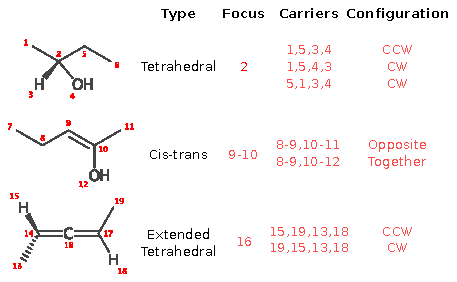
\includegraphics{img/stereodesc_annotated.pdf}
\label{fig:stereodatastructure}
\end{figure}




\begin{figure}[h!]
  \caption{\csentence{The raw input files of CHEMBL23970 and CHEMBL444314 are displayed (ChEMBL 21).}
    Without perceiving the stereochemistry indicated by Haworth
    projection in CHEMBL23970, the database entries are incorrectly
    considered distinct. Down stream aggregation databases mirror this
    separation (PubChem CID 5280, CID 65119).}
    \centering
    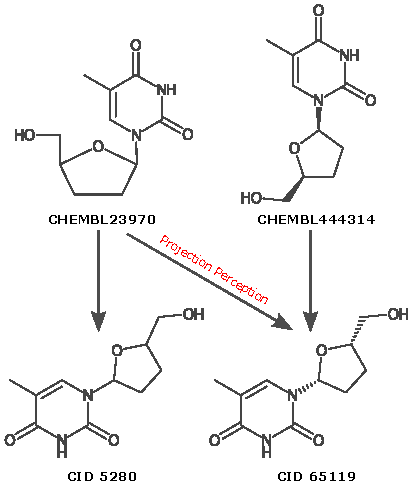
\includegraphics{img/projections_annotated.pdf}
    \label{fig:stereoprojections}
\end{figure}

\begin{figure}[h!]
  \caption{\csentence{Integrated example showing the rendering and SMILES
      parsing functionality. Example from U.S. Patent \textbf{US 2014 231770 A1} para 287.}}
  \centering
  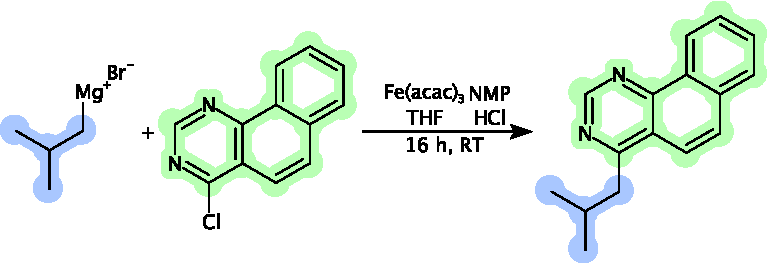
\includegraphics[width=\textwidth]{img/US20140231770A1_0287.pdf}
  \label{fig:depiction}
\end{figure}

\begin{figure}[h!]
  \caption{\csentence{{The improved structure diagram generation has improved
        code to solve overlap.}}
    The original SDG code used general heuristics (left) and the
    OverlapResolver would fine tune the layout to ensure atoms would not be placed
    at the same location (middle). The new SDG algorithm is able to
    make more rigorous changes, making the final output must more pleasing
    (right).}
    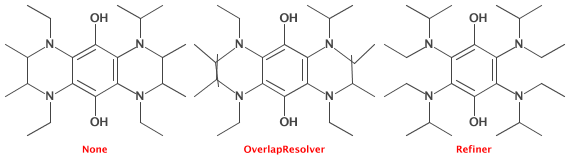
\includegraphics[width=\textwidth]{sdg.png}
    \label{fig:sdg}
\end{figure}

\begin{figure}[h!]
  \caption{\csentence{Structure diagram generation for structures with
      double bond and tetrahedral stereochemistry.}}
  \centering
  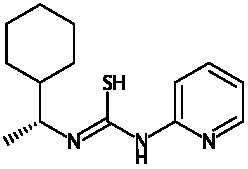
\includegraphics[width=0.3\textwidth]{sdg2.pdf}
  \label{fig:sdgstereo}
\end{figure}


\begin{figure}[h!]
  \caption{\csentence{Dependencies between CDK modules.}
    Visualization of the dependencies between CDK modules. For example,
    the cdk-core depends on the cdk-interfaces module. A few higher level
    modules have been left out: cdk-builder3dtools, cdk-legacy, and
    cdk-depict.}
  \centering
  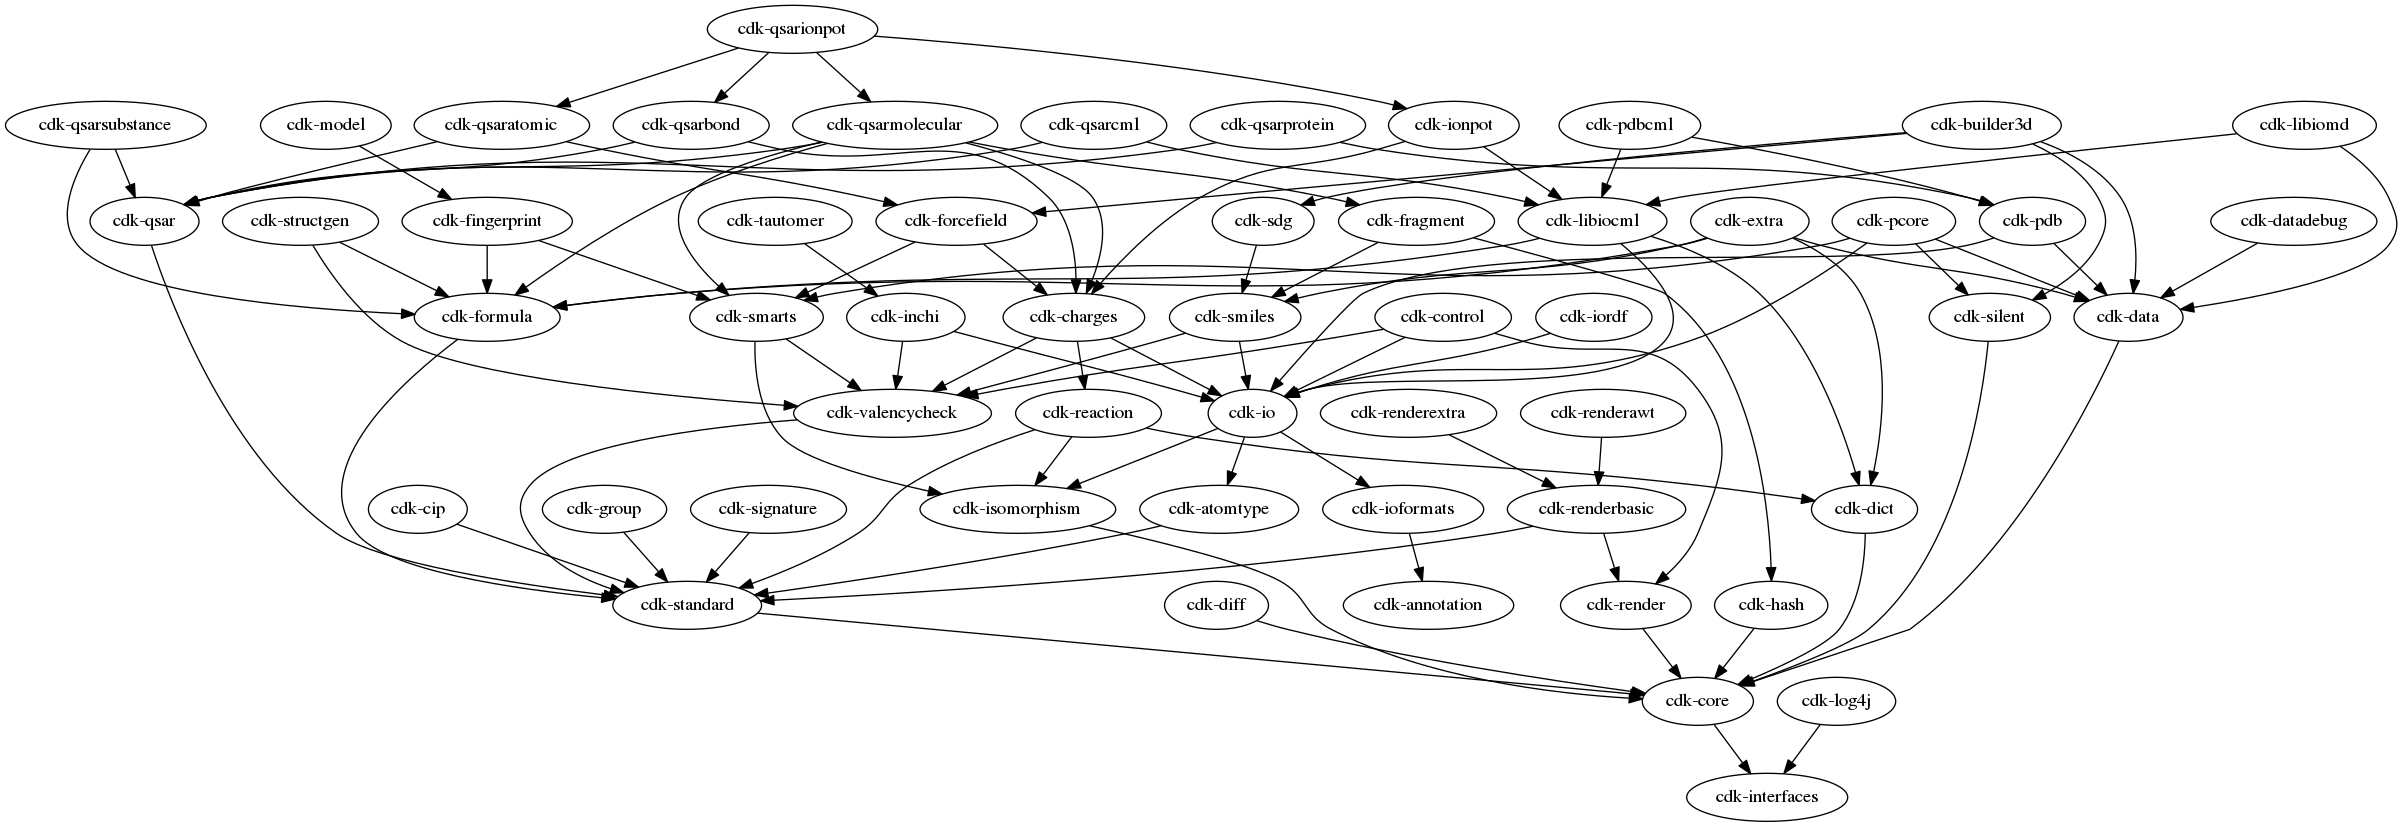
\includegraphics[width=\textwidth]{cdkDeps.png}
  \label{fig:deps}
\end{figure}

\begin{figure}[h!]
  \caption{\csentence{Examples of Sgroups now captured by the CDK and
      encoded in molfiles and CXSMILES. a) Ethyl esterification fully
      expanded reaction. b) Using Sgroup abbreviations allows display
      short cuts and more compact depiction. c) An example of a
      structure repeat unit in \textit{DNA 5'-phosphate}
      (\textbf{CHEBI:4294})}}
  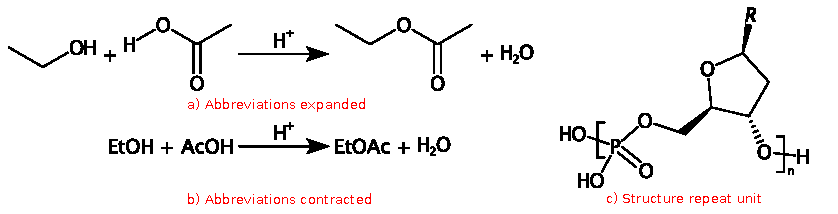
\includegraphics[width=\textwidth]{img/sgroups.pdf}
  \label{fig:sgroups}
\end{figure}
      




%%%%%%%%%%%%%%%%%%%%%%%%%%%%%%%%%%%
%% Tables                        %%

\clearpage

%% Use of \listoftables is discouraged.
%%
\section*{Tables}


  \subsection*{Table 1 - Evaluation of molecular formula generators.}
  \label{tab:formula_generators}
  The resulting formula counts and runtimes of the HR2, PFG, and CDK chemical
formula generators on two different inputs with two different mass tolerance
settings. For the set of small masses, 10,000 mass values in the range of
0--500 Da were randomly selected from the Global Natural Products Social
Molecular Networking database~\cite{wang2016}. For the set of large masses, 20
mass values in the range of 1,500--3,500 Da were randomly selected from the same
database. Formulas were generated using chemical elements C,H,N,O,P,S without
bounds (the allowed atom count was set to 0--10,000 for each element). All
heuristic filtering rules were disabled for the purpose of the evaluation. The
slight differences in the number of generated formulas were caused by different
isotope masses embedded in each software and/or by rounding errors during
calculation. The runtimes are average values from three independent runs
performed on three different 16-core Intel Xeon 2.9~GHz CPU workstations
equipped with 189~GB RAM, running Ubuntu Linux version 12.04.5 LTS and OpenJDK
Java runtime version 1.7.0\_101.
  \vskip 1\baselineskip

    \begin{minipage}{1\textwidth}
    \centering
    \begin{tabular}{llllllll}
	\multirow{2}{1in}{ Input } & \multirow{2}{1in}{ Mass tolerance ($\pm$ Da) } & \multicolumn{3}{c}{ \# of generated formulas } & \multicolumn{3}{c}{ Runtime (s) } \\
	& & HR2 & PFG & CDK & HR2 & PFG & CDK \\
	10,000 small masses & 0.001 & 616,846 & 616,846 & 616,843 & 669 & 168 & \textbf{41} \\
	10,000 small masses & 0.01 & 6,163,303 & 6,163,302 & 6,163,326 & 689 & 501 & \textbf{212} \\
	20 large masses & 0.001 & 4,912,939 & 4,912,939 & 4,912,904 & 26,370 & 1,292 & \textbf{177} \\
	20 large masses & 0.01 & 49,128,811 & 49,128,810 & 49,128,815 & 26,587 & 3,406 & \textbf{1,580} \\
    \end{tabular}
    \end{minipage}

    %% CTfile Format Support
%% To tabulate, r=read, w=write
      \subsection*{Table 2 - CTfile Format Support.}\label{tab:ctfileFormats}

    \begin{minipage}{1\textwidth}
    \renewcommand*{\thempfootnote}{\fnsymbol{mpfootnote}}
    \centering
    \begin{tabular}{lll}
  \textbf{Format}            & \textbf{V2000}  & \textbf{V3000} \\ \hline
    MOLfile & read and write & read and write \\
    RXNfile & read and write & read \\
    SDfile MOLfile & read and write & read \\ % FIXME: RGfile=n/a
    RGfile & read and write & \\
    RDfile & & \\ % FIXME: yes, we do have support
    \end{tabular}
    \end{minipage}


  \subsection*{Table 3 - The molecular fingerprints in CDK.}
  \label{tab:fingerprints}
  Listed are the currently available molecular fingerprint in CDK with
  information about whether they come as a bit and/or count version, what CDK version
  they were introduced in, their default size, and relevant
  references, where applicable.
  \vskip 1\baselineskip

    \begin{minipage}{1\textwidth}
    \renewcommand*{\thempfootnote}{\fnsymbol{mpfootnote}}
    \centering
    \begin{tabular}{lcclc}
                             & Bit version  & Count version & CDK version & Default Size    \\
  CircularFingerprinter~\cite{rogers2010extended, Clark2014}      & $\checkmark$ & $\checkmark$  & \cdkversion{}     & $1\,024$ / $2^{32}$%
\footnote[1]{For the CircularFingerprinter the bit version is folded to 1024 whereas the count version is unfolded.} \\
  EStateFingerprinter~\cite{Hall1995}       & $\checkmark$ &               & 1.2.0       & $79$            \\
  ExtendedFingerprinter      & $\checkmark$ &               & 1.0         & $1\,024$        \\
  Fingerprinter              & $\checkmark$ &               & 1.0         & $1\,024$        \\
  GraphOnlyFingerprinter     & $\checkmark$ &               & 1.0         & $1\,024$        \\
  HybridizationFingerprinter & $\checkmark$ &               & 1.4.0       & $1\,024$        \\
  KlekotaRothFingerprinter~\cite{Klekota2008}   & $\checkmark$ &               & 1.4.6       & $4\,860$        \\
  LingoFingerprinter~\cite{vidal2005lingo}         & $\checkmark$ &               & \cdkversion{}     & NA%
\footnote[2]{The LingoFingerprinter does not have a default size.}
                                                                                             \\
  MACCSFingerprinter         & $\checkmark$ &               & 1.2.0       & $166$           \\
  PubchemFingerprinter~\cite{pubchemFP}       & $\checkmark$ &               & 1.4.0       & $881$            \\
  ShortestPathFingerprinter  & $\checkmark$ &               & \cdkversion{}     & $1\,024$        \\
  SignatureFingerprinter~\cite{signaturefingerprints}     & $\checkmark$ & $\checkmark$  & \cdkversion{}     & $2^{32}$         \\
  SubstructureFingerprinter  & $\checkmark$ &               & 1.0         & $307$           \\

    \end{tabular}
    \end{minipage}

\newpage
    
      \subsection*{Table 4 - A selection of key CDK modules with major changes.}\label{tab:modules}
  An overview of a selection of often used CDK modules with description,
  dependencies on third-party libraries, and the major changes since
  version~1.2. Dependencies between modules are depicted in Figure~\ref{fig:deps}.
  \vskip 1\baselineskip

    \begin{minipage}{1\textwidth}
    \renewcommand*{\thempfootnote}{\fnsymbol{mpfootnote}}
    \centering
    \begin{tabular}{lp{3cm}p{3cm}l}
  \textbf{Module}            & \textbf{Description}  & \textbf{Major Changes} & \textbf{Dependencies} \\ \hline
  interfaces                 & Interfaces for the data models. & & Vecmath 1.5.2 \\ \hline
  core                       & Core functionality.             & & Google Guava 17.0 \\ \hline % FIXME: how to add https://github.com/google/guava ?
  standard                   & Common functionality.           & & \\ \hline
  render                     & Graphical rendering.            & Redesigned to make it more modular and support multiple widget toolkits, like AWT and SWT. & \\ \hline
  isomorphism                & Isomorphism and substructure searching. & & \\ \hline
  atomtype                   & Various non-core atom type schemes.     & Unified approach where atom typing is separated from other algorithms. & \\ \hline
  ioformats                  & Definitions of (chemical) input/output formats. & & \\ \hline
  io                         & Readers and writers for input/output formats.  & The molfile reader has been rewritten and supports in atom types defind in the specification. & XPP3 1.1.4c \\ \hline
  iordf                      & Stores data models as in the Resource Description Framework serialization formats. & New. & Jena 2.7.4 \\ \hline
  inchi                      & IUPAC International Chemical Identifier support. & & JNI-InChI 0.8~\cite{Spjuth2013}  \\ \hline
  libiocml                   & Writer for the Chemical Markup Language format. & & XOM 1.2.5, CMLXOM 3.1~\cite{Murray-Rust2011} \\ \hline
  sdg                        & Structure diagram generation.  & Much improved overlap resolution. & \\ \hline
  smiles                     & Reading and writing in the SMILES format. & SMILES support performance and coverage is greatly improved. & Beam 0.9.1~\cite{Beam} \\ \hline
  smarts                     & Substructure searching with the SMARTS format. & & Beam 0.9.1~\cite{Beam} \\ \hline
  hash                       & Molecular hash codes~\cite{Ihlenfeldt94}. & & \\ \hline
  formula                    & Chemical formula support. & New. & \\ \hline
  fingerprint                & Calculate fingerprints. & Many new fingerprint types (see text). & Apache Commons Math 3.1.1 \\ \hline
  qsar and qsarmolecular                       & Molecular descriptors.  & & XOM 1.2.5, JAMA 1.0.3~\cite{Hicklin2012} \\ \hline
  signatures                 & Calculation of molecular and atomic signatures. & & Signatures 1.1 \\ \hline
    \end{tabular}
    \end{minipage}


\subsection*{Table 5 - SMARTS matching performance.}\label{tab:smigrep}
  Total time taken to match the SMARTS \texttt{O=[C,N]aa[N,O;!H0]} against $\sim$1.5 million SMILES from
  ChEMBL 21. The reported time is for single core execution, measure with the Unix time utility (Cent OS 7, Intel Core i7-4790 CPU @ 3.60GHz). The times for recent versions of Open Babel~\cite{OBoyle2011} and RDKit~\cite{rdkit} are included for reference but this is not intended to be a systematic comparison. The difference in number found is due to variations in valence and aromaticity models.
  \vskip \baselineskip

\begin{tabular}{lll}
Toolkit                   & Time (s)   & Matched \\
\hline
CDK 1.4.9                 & 3,843  & 69,782  \\
CDK \cdkversion{}         & 67   & 62,518  \\
Open Babel 2.3.90         & 835 & 61,906  \\
RDKit 2016.3.4            & 378  & 62,402  \\
\end{tabular}


\end{backmatter}

\end{document}







